\problemname{Rabbit Holes}

In the recently concluded competition Databävern \href{www.databavern.se}{(see website)},
the students saw an example of the curious interplay of animals:

A group of $N$ beavers is going for a walk in the forest. They walk in a line, one
after another. But the mischievous rabbits have dug a bunch of holes along the path the beavers walk on.

The holes are deep enough for a certain number of beavers to fall in. When
the hole is full of beavers, the beavers behind can pass on top of
the beavers in the hole, until finally the last beaver in the line pulls the beavers out of
the hole, the top one first and the bottom one last. That is, if we have five beavers (5
4 3 2 1) walking to the right (number 1 is first and number 5 is last in
the line), and they come to a hole where three beavers fit, the following would happen:

\begin{figure}[ht!]
\centering
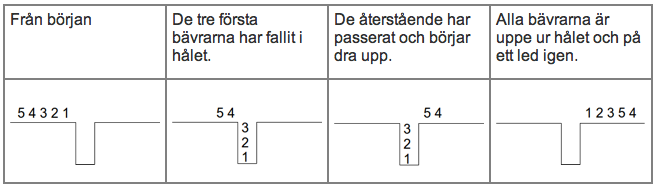
\includegraphics[width=0.7\textwidth]{kaninhol.png}
\caption{An illustration of a rabbit hole and how the beavers walk over the hole.}
\label{overflow}
\end{figure}

Now imagine that the rabbits have made three holes on the path (each with a depth
between $1$ and $N-1$). Write a program that, given the order of the line after
the beavers have passed all holes, computes the depth of each hole.

\section*{Input}

The first line contains an integer $N$, the number of beavers, where $2 \leq N \leq 10$. The second line
contains $N$ distinct integers, each between 1 and N. These describe the order of
the beavers after they have passed the three rabbit holes. The initial order is $N$, $N-1$,
$N-2,\ldots,1$. Note that they walk to the right, so beaver $1$ is first in the line.

\section*{Output}

Three integers between $1$ and $N-1$, the depth of the first, second, and third
rabbit hole, respectively. You may assume that there is exactly one solution for each given
test case.
